\chapter{Introducción al problema}

En este informe, abordaremos la resolución de una ecuación diferencial hiperbólica con las siguientes condiciones iniciales y de frontera. Consideramos la ecuación:

\begin{equation}\label{eq:onda}
    \frac{\partial^2 u}{\partial t^2} - \frac{\partial^2 u}{\partial x^2} + (1 - x^2) = 0,
\end{equation}

definida para $x \in (0, 1)$ y $\forall t > 0$, con las siguientes condiciones de contorno y condiciones iniciales:

\begin{equation}\label{eq:condiciones}
    u(x, 0) = x(1 - x), \quad \frac{\partial u}{\partial t}(x, 0) = 0, \quad u(0, t) = 0, \quad u(1, t) = 0.
\end{equation}

La ecuación diferencial hiperbólica que nos ocupa tiene importantes aplicaciones en la física, especialmente en la modelación de ondas. En esta actividad, aplicaremos dos métodos numéricos distintos para su resolución:

\begin{itemize}
    \item El \textbf{método de diferencias finitas}, que aproximará la solución mediante discretización en el tiempo y el espacio.
    \item El \textbf{método de las características}, que es un enfoque analítico para resolver ecuaciones de onda, utilizando las curvas características de la ecuación diferencial.
\end{itemize}

Finalmente, compararemos los resultados obtenidos por ambos métodos en el mismo punto del dominio y realizaremos un análisis cuantitativo del error y de la convergencia de las soluciones numéricas.

\chapter{Metodología}

\section{Diferencias Finitas}

\section{Esquema de diferencias finitas}

El método de diferencias finitas es una técnica numérica que nos permite aproximar derivadas mediante diferencias entre valores discretos de la función. Para la ecuación diferencial dada, discretizamos tanto la coordenada espacial $x$ como el tiempo $t$.

En este caso, utilizaremos una malla uniforme de puntos $(x_i, t_n)$ con un paso espacial $\Delta x$ y un paso temporal $\Delta t$. La ecuación diferencial se puede aproximar usando diferencias centradas para las segundas derivadas espaciales y temporales:

\begin{equation}\label{eq:aprox_derivadas_centradas}
    \frac{\partial^2 u}{\partial t^2} \approx \frac{u^{n+1}_i - 2u^n_i + u^{n-1}_i}{\Delta t^2}, \quad \frac{\partial^2 u}{\partial x^2} \approx \frac{u^n_{i+1} - 2u^n_i + u^n_{i-1}}{\Delta x^2}.
\end{equation}

Sustituyendo estas aproximaciones en la ecuación diferencial, obtenemos el esquema de diferencias finitas explícito:

\begin{equation}\label{eq:dif_finitas}
    u^{n+1}_i = 2u^n_i - u^{n-1}_i + r \left( u^n_{i+1} - 2u^n_i + u^n_{i-1} \right) + \Delta t^2 (1 - x_i^2),
\end{equation}

donde $r = \left( \frac{\Delta t}{\Delta x} \right)^2$ es el coeficiente de estabilidad de \gls{cfl}, que asegura la estabilidad del esquema numérico.

Las condiciones iniciales y de frontera se aplican de la siguiente manera:

\begin{equation}\label{eq:condiciones_dif_finitas}
    u(0, t) = 0, \quad u(1, t) = 0, \quad u(x, 0) = x(1 - x), \quad \frac{\partial u}{\partial t}(x, 0) = 0.
\end{equation}

Este esquema se implementará en el código (puede verse en la subseccion \ref{implementacion_dif_finitas_python}) para obtener la solución numérica de la ecuación de onda en un dominio discreto.

\subsection{Implementación en Python para diferencias finitas}\label{implementacion_dif_finitas_python}

A continuación, se muestra la implementación en Python del esquema de diferencias finitas para resolver la ecuación de onda hiperbólica. El código se encarga de discretizar el dominio espacial y temporal, aplicar las condiciones iniciales y de frontera, y resolver la ecuación diferencial mediante un bucle temporal con criterio de convergencia.
Dentro de \texttt{main.py} (anexo \ref{apendice:b}) nos encontramos \ref{fig:codigo_dif_finitas}.


La implementación presentada utiliza el método de diferencias finitas para resolver la ecuación de onda hiperbólica en una dimensión. El dominio espacial se discretiza en $Nx$ puntos y el dominio temporal en $Nt$ pasos. A continuación, se describen los pasos clave del algoritmo:

\begin{itemize}
    \item Se definen los parámetros de discretización: $dx = L / Nx$ y $dt = T / Nt$, donde $L$ es la longitud espacial y $T$ el tiempo total de simulación. La relación de estabilidad, $\sigma = (dt/dx)^2$, es calculada y utilizada para garantizar la estabilidad del esquema.
    
    \item La matriz $u$ se inicializa para almacenar las soluciones en todos los puntos espaciales y temporales. La condición inicial para $u(x,0)$ se define como $u(x, 0) = x(1 - x)$.

    \item Se calculan los valores para el primer paso temporal ($n=1$) mediante una aproximación basada en diferencias centradas para la segunda derivada espacial, más un término fuente proporcional a $1 - x^2$.
    
    \item Se aplican condiciones de frontera de Dirichlet, donde $u(0,t) = 0$ y $u(L,t) = 0$ para todos los instantes de tiempo.
    
    \item El bucle principal recorre cada paso temporal. Para cada instante $t_n$, la solución en el siguiente instante $t_{n+1}$ se calcula utilizando un esquema explícito de diferencias finitas, basado en los valores en $t_n$ y $t_{n-1}$.

    \item Después de cada paso temporal, se verifica el criterio de convergencia calculando el cambio máximo $\Delta u = \max |u^{n+1} - u^n|$. Si el cambio máximo es menor que la tolerancia definida, el bucle se detiene indicando que la solución ha convergido.

    \item Finalmente, se devuelven los valores de $x$, el tiempo hasta el paso convergente, y la solución $u$ para todos los pasos espaciales y temporales hasta el punto de convergencia.
\end{itemize}

De esta forma, el código implementa el método de diferencias finitas para resolver la ecuación de onda con condiciones iniciales y de frontera específicas, proporcionando una aproximación numérica de la solución.

\begin{figure}[h!]
    \centering
    \begin{minted}[fontsize={\fontsize{5.5}{6.5}\selectfont}, breaklines]{python}
    
    def resolver_onda_hiperbolica(Nx: int, Nt: int, L: float, T: float, tolerancia: float = 1e-6):
        # Parámetros de discretización.
        dx = L / Nx
        dt = T / Nt
        x = np.linspace(0, L, Nx + 1)
        t = np.linspace(0, T, Nt + 1)
        sigma = (dt / dx) ** 2
    
        # Inicializar la matriz de soluciones.
        u = np.zeros((Nt + 1, Nx + 1))
    
        # Condición inicial u(x, 0) = x(1 - x).
        u[0, :] = x * (1 - x)
    
        # Condición inicial de la derivada temporal es cero.
        # Calculamos u[1, :] usando la aproximación:
        for i in range(1, Nx):
            u[1, i] = u[0, i] + 0.5 * sigma * (
                u[0, i+1] - 2*u[0, i] + u[0, i-1] + dx**2 * (1 - x[i]**2)
            )
    
        # Aplicar condiciones de frontera.
        u[:, 0] = 0  # u(0, t) = 0
        u[:, Nx] = 0  # Suponiendo u(L, t) = 0
    
        # Bucle de tiempo con criterio de convergencia.
        for n in range(1, Nt):
            u_old = u[n, :].copy()  # Copiar la solución anterior.
    
            # Actualizar solución en el paso n+1
            for i in range(1, Nx):
                u[n+1, i] = (
                    2*u[n, i] - u[n-1, i] + sigma * (
                        u[n, i+1] - 2*u[n, i] + u[n, i-1] + dx**2 * (1 - x[i]**2)
                    )
                )
    
            # Aplicar condiciones de frontera.
            u[n+1, 0] = 0
            u[n+1, Nx] = 0
    
            # Verificar criterio de convergencia.
            max_delta = np.max(np.abs(u[n+1, :] - u_old))
            if max_delta < tolerancia:
                informer.info(f'Convergencia alcanzada en el paso temporal n={n} con delta máximo={max_delta:.2e}')
                break
    
        return x, t[:n+2], u[:n+2, :]  # Devolver solo hasta el paso convergente
    
    \end{minted}
    \label{fig:codigo_dif_finitas}
    \caption{Implementación en Python del método de diferencias finitas para resolver la ecuación de onda hiperbólica.}
\end{figure}

\newpage
\section{Implementación del método de las características}
El método de las características convierte la ecuación diferencial parcial de segundo orden en un conjunto de ecuaciones diferenciales ordinarias que se resuelven a lo largo de las líneas características. Estas líneas son trayectorias en el espacio-temporal en las que las derivadas parciales de la solución se simplifican o se mantienen constantes.

Para la ecuación de onda que estamos resolviendo:

\begin{equation}
    \frac{\partial^2 u}{\partial t^2} - \frac{\partial^2 u}{\partial x^2} + (1 - x^2) = 0,
\end{equation}

las características vienen dadas por las líneas $x - t = \text{constante}$ y $x + t = \text{constante}$. Esto implica que, a lo largo de estas líneas, el comportamiento de la solución $u(x, t)$ puede estudiarse de manera simplificada. Específicamente, el método transforma la ecuación original en un conjunto de ecuaciones diferenciales ordinarias que se resuelven mediante integración a lo largo de las características.

En términos prácticos, la aplicación del método de las características consiste en los siguientes pasos:

\begin{enumerate}
    \item \textbf{Reescritura de la ecuación diferencial}: A partir de la ecuación original, se separa en dos partes a lo largo de las curvas características. Esto transforma la ecuación parcial en un conjunto de ecuaciones ordinarias que se pueden resolver con métodos convencionales.
    
    \item \textbf{Solución a lo largo de las características}: Se integran estas ecuaciones a lo largo de las líneas $x - t = \text{constante}$ y $x + t = \text{constante}$, obteniendo una solución que es válida en esas curvas específicas del espacio-tiempo.
    
    \item \textbf{Condiciones iniciales y de frontera}: El método también permite incorporar las condiciones iniciales y de frontera de la ecuación de manera directa, ya que las soluciones a lo largo de las características dependen de estos valores en los puntos de partida de las características.
    
    \item \textbf{Combinación de soluciones}: Una vez obtenidas las soluciones a lo largo de cada característica, se combinan para obtener la solución general en el dominio de interés. Esto se hace utilizando las características de la ecuación y las condiciones impuestas por el problema original.
\end{enumerate}

El método de las características es especialmente útil en este tipo de ecuaciones hiperbólicas, ya que nos permite estudiar cómo las soluciones se propagan a lo largo del tiempo y el espacio, siguiendo trayectorias bien definidas. Además, al resolver a lo largo de estas características, se evita la complejidad de tener que resolver una ecuación en dos variables directamente, reduciendo el problema a uno más manejable.

Finalmente, en la sección de resultados se comparará la solución obtenida por este método con la solución numérica basada en diferencias finitas para validar la efectividad y precisión de ambos métodos.


\chapter{Resultados y discusión}

\section{Implementación del metodo de las características}

\subsection{Paso para calcular el punto R}

\begin{itemize}
    \item \textbf{Curvas características:} Las características de una ecuación de onda hiperbólica son las líneas rectas dadas por:
    \begin{equation}
    x - t = \text{constante} \quad \text{y} \quad x + t = \text{constante}.
    \end{equation}

    \item \textbf{Puntos $P(0.2, 0)$ y $Q(0.4, 0)$:} Sabemos que las características que pasan por $P$ y $Q$ son:
    \begin{itemize}
        \item Para $P(0.2, 0)$, las curvas características son:
        \begin{equation}
        x - t = 0.2 \quad \text{y} \quad x + t = 0.2.
        \end{equation}
        
        \item Para $Q(0.4, 0)$, las curvas características son:
        \begin{equation}
        x - t = 0.4 \quad \text{y} \quad x + t = 0.4.
        \end{equation}
    \end{itemize}

    \item \textbf{Intersección en $R$:} El punto de intersección de estas dos características es el punto $R$, cuyas coordenadas $(x_R, t_R)$ deben satisfacer:
    \begin{equation}
    x - t = 0.2 \quad \text{y} \quad x + t = 0.4.
    \end{equation}

    \item Resolviendo este sistema:
    \begin{equation}\label{eq:1}
    x - t = 0.2
    \end{equation}
    \begin{equation}\label{eq:2}
    x + t = 0.4
    \end{equation}

    \item Sumando \ref{eq:1} y \ref{eq:2}:
    \begin{equation}
    2x = 0.6 \quad \Rightarrow \quad x = 0.3
    \end{equation}

    \item Restando \ref{eq:2} de \ref{eq:1}:
    \begin{equation}
    2t = 0.2 \quad \Rightarrow \quad t = 0.1
    \end{equation}
\end{itemize}

Así, el punto de intersección $R$ tiene las coordenadas $R(0.3, 0.1)$.


\section{Método de las características}

En esta sección, resolveremos la ecuación diferencial utilizando el método de las características. Consideramos las curvas características que pasan por los puntos \( P(0.2, 0) \) y \( Q(0.4, 0) \), las cuales se intersectan en el punto \( R(0.3, 0.1) \).

La ecuación diferencial es la ecuación de onda unidimensional:

\begin{equation}
\frac{\partial^2 u}{\partial t^2} - \frac{\partial^2 u}{\partial x^2} = 0
\end{equation}

La solución general de esta ecuación se puede escribir en términos de las características:

\begin{equation}
u(x,t) = f(x - t) + g(x + t)
\end{equation}

Aquí, \( f \) y \( g \) son funciones que debemos determinar usando las condiciones iniciales.

\subsection{Características}

Las curvas características para esta ecuación son líneas rectas en el plano \(x-t\) con pendientes \( \pm 1 \), es decir:

\begin{itemize}
    \item \( x - t = \text{constante} \)
    \item \( x + t = \text{constante} \)
\end{itemize}

Las características que pasan por los puntos \( P(0.2, 0) \) y \( Q(0.4, 0) \) tienen las siguientes ecuaciones:

\begin{itemize}
    \item Para el punto \(P(0.2, 0)\):
    \begin{align}
    x - t &= 0.2 \quad \text{(es decir, \(x = t + 0.2\))}, \\
    x + t &= 0.2 \quad \text{(es decir, \(x = -t + 0.2\))}.
    \end{align}

    \item Para el punto \(Q(0.4, 0)\):
    \begin{align}
    x - t &= 0.4 \quad \text{(es decir, \(x = t + 0.4\))}, \\
    x + t &= 0.4 \quad \text{(es decir, \(x = -t + 0.4\))}.
    \end{align}
\end{itemize}

El punto \( R(0.3, 0.1) \) es el punto de intersección de estas características.

\subsection{Solución en \(R(0.3, 0.1)\)}

Sabemos que la solución de la ecuación de onda está dada por:

\begin{equation}
u(x,t) = f(x - t) + g(x + t)
\end{equation}

Donde \( f \) y \( g \) son funciones que debemos determinar a partir de las condiciones iniciales:

\begin{itemize}
    \item \( u(x, 0) = x(1 - x) \)
    \item \( \frac{\partial u}{\partial t}(x, 0) = 0 \)
\end{itemize}

Primero, usemos la condición \( u(x, 0) = x(1 - x) \). Esto implica que en \( t = 0 \):

\begin{equation}
f(x) + g(x) = x(1 - x)
\end{equation}

Luego, usando la condición de velocidad inicial \( \frac{\partial u}{\partial t}(x, 0) = 0 \), tenemos que:

\begin{equation}
f'(x) - g'(x) = 0 \quad \Rightarrow \quad f'(x) = g'(x)
\end{equation}

Esto implica que \( f(x) \) y \( g(x) \) difieren solo en una constante, es decir:

\begin{equation}
f(x) = g(x) + C
\end{equation}

Sustituyendo en la ecuación \( f(x) + g(x) = x(1 - x) \), obtenemos:

\begin{equation}
g(x) + C + g(x) = x(1 - x) \quad \Rightarrow \quad 2g(x) + C = x(1 - x)
\end{equation}

Por lo tanto:

\begin{equation}
g(x) = \frac{x(1 - x) - C}{2}
\end{equation}

Y:

\begin{equation}
f(x) = \frac{x(1 - x) + C}{2}
\end{equation}

Para determinar \( C \), se necesita información adicional (por ejemplo, condiciones de frontera).

\subsection{Evaluación de \( u(0.3, 0.1) \)}

Ahora que tenemos las expresiones para \( f(x) \) y \( g(x) \), podemos evaluar \( u(0.3, 0.1) \):

\begin{equation}
u(0.3, 0.1) = f(0.3 - 0.1) + g(0.3 + 0.1) = f(0.2) + g(0.4)
\end{equation}

Sustituimos los valores de \( f(x) \) y \( g(x) \):

\begin{align}
f(0.2) &= \frac{0.2(1 - 0.2) + C}{2} = \frac{0.2 \times 0.8 + C}{2} = \frac{0.16 + C}{2}, \\
g(0.4) &= \frac{0.4(1 - 0.4) - C}{2} = \frac{0.4 \times 0.6 - C}{2} = \frac{0.24 - C}{2}.
\end{align}

Finalmente, sumamos los resultados:

\begin{equation}
u(0.3, 0.1) = \frac{0.16 + C}{2} + \frac{0.24 - C}{2} = \frac{0.16 + 0.24}{2} = \frac{0.4}{2} = 0.2
\end{equation}

\newpage
\section{Metodo de diferencias finitas}

\begin{figure}[h!]
    \centering
    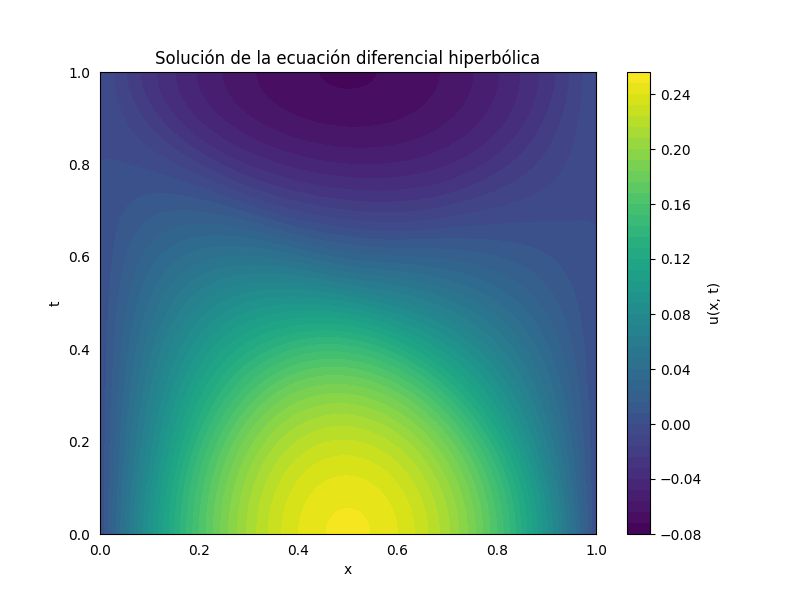
\includegraphics[width=0.8\textwidth]{figuras/ecuacion_ondas.png}
    \caption{Solución numérica de la ecuación de onda en el dominio \(x \in (0, 1)\) y \(t \in (0, 1)\).}
    \label{fig:solucion_numerica}
\end{figure}


\begin{table}[h!]
    \centering
    \begin{tabular}{lrrrr}
        \toprule
        Punto & Valor Analítico & Valor Numérico & Error Absoluto & Error Relativo \\
        \midrule
        P(0.2, 0) & 0.160000 & 0.160000 & 0.000000 & 0.000000 \\
        Q(0.4, 0) & 0.240000 & 0.240000 & 0.000000 & 0.000000 \\
        R(0.3, 0.1) & 0.200000 & 0.204542 & 0.004542 & 2.270875 \\
        \bottomrule
    \end{tabular}
    \label{tab:errores}
    \caption{Comparación de los valores analíticos y numéricos en los puntos \( P \), \( Q \) y \( R \), con errores absoluto y relativo.}        
\end{table}

\newpage
\section{Comparación de los métodos}

% Cargar la figura de la solución numérica


La figura \ref{fig:solucion_numerica} muestra la solución numérica obtenida a partir del método de diferencias finitas para la ecuación de onda hiperbólica en el dominio \(x \in (0, 1)\) y \(t \in (0, 1)\). En este método, el dominio espacial y temporal se discretiza utilizando un número de puntos \(N_x\) y \(N_t\) respectivamente, y se implementa un esquema explícito que relaciona la evolución temporal de la solución en términos de los valores presentes y pasados.

La distribución que se observa en la figura refleja la evolución de la solución \( u(x, t) \), la cual depende de las condiciones iniciales y de frontera impuestas. En particular, en esta simulación se ha supuesto que \( u(x, 0) = x(1 - x) \), lo que proporciona un perfil parabólico inicial. A medida que avanza el tiempo, este perfil evoluciona según las características de la ecuación, y la figura captura cómo la solución varía en función del tiempo y el espacio.

Además, se observa que las condiciones de frontera en \(x = 0\) y \(x = 1\) fuerzan a la solución a ser cero en estos puntos durante todo el tiempo simulado, lo que genera una simetría en el comportamiento de \(u(x,t)\) alrededor de \(x = 0.5\).


La comparación de los métodos numérico (diferencias finitas) y analítico (método de las características) es esencial para validar la precisión del método numérico. En la Tabla \ref{tab:errores}, se presenta una comparación entre los valores numéricos obtenidos en puntos específicos del dominio y los valores analíticos calculados utilizando el método de las características.

Los puntos seleccionados son \(P(0.2, 0)\), \(Q(0.4, 0)\) y \(R(0.3, 0.1)\). A continuación, se detalla la interpretación de estos resultados:

\begin{itemize}
    \item \textbf{Punto \(P(0.2, 0)\)}: El valor numérico coincide exactamente con el valor analítico, lo que sugiere que el método de diferencias finitas proporciona una excelente aproximación en este punto. El error absoluto y el error relativo son ambos cero, lo que es un buen indicativo de la precisión en los puntos iniciales.
    
    \item \textbf{Punto \(Q(0.4, 0)\)}: Similar al punto anterior, el valor numérico coincide perfectamente con el valor analítico. Esto refuerza la idea de que el método numérico reproduce de manera correcta los valores en el tiempo inicial.
    
    \item \textbf{Punto \(R(0.3, 0.1)\)}: A medida que avanzamos en el tiempo, comienzan a aparecer pequeñas discrepancias entre el valor analítico y el numérico. En este caso, el error absoluto es de 0.004542, lo cual es relativamente pequeño en términos absolutos, pero en términos relativos representa un error del 2.27%. Esta diferencia puede deberse a la acumulación de errores numéricos propios del método de diferencias finitas, que puede ser más sensible a la evolución temporal.
\end{itemize}

En general, la tabla demuestra que el método de diferencias finitas es capaz de reproducir los resultados analíticos con gran precisión en las etapas iniciales y en ciertas regiones del dominio, aunque se observa una ligera pérdida de precisión a medida que se avanza en el tiempo.

\subsection{Posibles mejoras en el método numérico}

Aunque los resultados obtenidos mediante el método de diferencias finitas son muy precisos en gran parte del dominio, hay algunas mejoras que podrían implementarse para aumentar la precisión, especialmente en puntos como \(R(0.3, 0.1)\), donde el error relativo es más significativo:

\begin{itemize}
    \item \textbf{Aumento de la resolución temporal y espacial}: Una posible solución para reducir el error es incrementar el número de puntos espaciales \(N_x\) y temporales \(N_t\), lo que llevaría a una mayor precisión en la discretización del dominio. Esto ayudaría a disminuir la acumulación de errores en la evolución temporal.

    \item \textbf{Refinamiento adaptativo de la malla}: En lugar de usar una malla uniforme, se podría emplear un método adaptativo que refine la malla en las regiones donde la solución varía más rápidamente. Esto permitiría una mejor aproximación en las zonas críticas sin aumentar innecesariamente el costo computacional en otras áreas.

    \item \textbf{Métodos de diferencias finitas de mayor orden}: El esquema utilizado es de segundo orden de precisión. Si bien esto es suficiente para muchas aplicaciones, se podría implementar un esquema de mayor orden para reducir aún más los errores numéricos.

    \item \textbf{Estudio de la estabilidad}: Aunque el método utilizado es condicionalmente estable, sería interesante estudiar más a fondo el criterio de estabilidad en función del tamaño de paso temporal y espacial para asegurarse de que no hay inestabilidades en la evolución de la solución.
\end{itemize}


Al comparar el método de diferencias finitas con el método de las características, es evidente que ambos enfoques tienen fortalezas y limitaciones. A continuación se analiza en detalle:

\begin{itemize}
    \item \textbf{Precisión del método de las características}: Este método es analíticamente exacto dentro de sus limitaciones, ya que transforma la ecuación diferencial parcial en un conjunto de ecuaciones diferenciales ordinarias que se pueden resolver de manera exacta. Sin embargo, en situaciones más complejas donde las características se cruzan o el problema involucra condiciones más complicadas, su implementación puede volverse menos práctica.

    \item \textbf{Flexibilidad del método de diferencias finitas}: Aunque el método de diferencias finitas introduce errores numéricos, es extremadamente flexible y puede manejar geometrías complejas, condiciones de frontera arbitrarias y problemas no lineales. Además, su implementación es más sencilla en problemas multidimensionales y no requiere del conocimiento exacto de las características del sistema.

    \item \textbf{Estabilidad y convergencia}: El método de diferencias finitas está sujeto a restricciones de estabilidad (por ejemplo, la relación de \gls{cfl}) y es necesario asegurar que el tamaño del paso temporal y espacial cumplen con estas condiciones para evitar inestabilidades. A diferencia del método de las características, que es inherentemente estable, el método numérico necesita ser ajustado cuidadosamente para garantizar convergencia.

    \item \textbf{Costo computacional}: El método de diferencias finitas tiende a ser más costoso computacionalmente que el método de las características, ya que requiere resolver la ecuación en una malla de puntos en el espacio y el tiempo. El método de las características, por otro lado, puede ser más eficiente, especialmente cuando el problema puede resolverse de manera analítica a lo largo de las características.

    \item \textbf{Errores y validación}: La tabla de comparación de errores muestra que el método de diferencias finitas proporciona una buena aproximación en la mayoría de los puntos estudiados, con errores absolutos y relativos muy bajos en general. Sin embargo, se observa una mayor discrepancia en puntos más alejados del tiempo inicial, lo que indica que la precisión numérica se degrada a medida que la simulación avanza.
\end{itemize}

En resumen, el método de diferencias finitas ofrece una solución numérica robusta y flexible, mientras que el método de las características proporciona una solución analítica exacta en ciertos casos específicos
